\documentclass[11pt]{article}
\usepackage[letterpaper, margin=1.1in]{geometry}
\usepackage{amssymb}
%\usepackage[ruled, vlined]{algorithm2e}
\usepackage{amsmath}
\usepackage{tikz}
\usetikzlibrary{calc}
\usepackage[font=footnotesize]{caption}
\usepackage{float}
\usepackage{mathtools}
\usepackage{mymath,gmech}

\newcommand{\TODO}[1]{\textcolor{red}{[TODO: #1]}}

\begin{document}

\newcommand{\RomanNumeralCaps}[1]
    {\MakeUppercase{\romannumeral #1}}

\newcommand{\imJacV}{\boldsymbol{L}}
\newcommand{\pointSetV}{\boldsymbol{q}}
\newcommand{\featSetV}{\boldsymbol{s}}
\newcommand{\featSetDV}{\boldsymbol{s}^*}
\newcommand{\error}{\boldsymbol{e}}

From the trajectory servoing control design in \S \RomanNumeralCaps{2}.C
\begin{equation} \label{eq:IBVStrajTrack}
  \omega = {\imJacV^2(\pointSetV^{\mc C},\featSetV)}^\dagger
    \bigg( \imJacV^1(\pointSetV^{\mc C^*}(t),\featSetDV(t)) \nu^* {(t)} 
          -\imJacV^1(\pointSetV^{\mc C},\featSetV) \nu
      + \imJacV^2(\pointSetV^{\mc C^*}(t),\featSetDV(t)) \omega^* {(t)}
      - \lambda \error \bigg),
\end{equation}
there is a control gain $\lambda$ affecting the tracking performance. 
We perform a set of simulations to tune the control gain that can give the 
best performance.
Five evaluation metrics: average lateral error (ALE), terminal error (TE), 
normalized path difference area (NPDA), 
angular normalized control effort (ANCE) and angular control smoothness (ACS).
The outcomes in the following tables are the averages over 
all trajectory templates.
The details about how to obtain these metrics can refer to another supplemental 
material in the same directory.

\TODO{add ale and double check if all values are up to date.}

\section{Short distance trajectory servoing}\label{sec:short}

In Table.\ref{tab:shortTune}, the first three rows evaluate the accuracy of 
trajectory tracking. The last two imply the performance of control signal.
When $\lambda=7$, the tracking accuracy is the best. Angular control effort 
has similar value to the lowest. The higher the control gain is, the less 
smoothness it has.
Therefore, for short distance trajectory experiments, 
we chose $\lambda=7$ to obtain the best accuracy 
and slightly sacrifice smoothness.

\begin{figure*}[h]
\begin{minipage}[t]{\textwidth}
\centering
%\vspace*{-1.45in}
\captionof{table}{ Control gain $\lambda$ tuning over short distance trajectories \label{tab:shortTune}}
\vspace*{-0.5em}
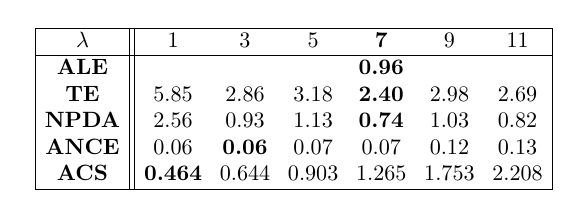
\begin{tikzpicture}[inner sep=0pt,outer sep=0pt,scale=1, every node/.style={scale=0.8}]
    % 
	\node[anchor=north west] (sim_tune) at (0, 0pt)
    {
    \setlength{\tabcolsep}{4pt}
    \begin{tabular}{|c||cccccc|}
    \hline 
    \textbf{$\lambda$} & 1 & 3 & 5 & \textbf{7} & 9 & 11 \\ 
    \hline 
    \textbf{ALE}  &  &  &  & \textbf{0.96} &  &  \\ 
    \textbf{TE}   & 5.85 & 2.86 & 3.18 & \textbf{2.40} & 2.98 & 2.69  \\ 
    \textbf{NPDA} & 2.56 & 0.93 & 1.13 & \textbf{0.74} & 1.03 & 0.82  \\ 
    \textbf{ANCE} & 0.06 & \textbf{0.06} & 0.07 & 0.07 & 0.12 & 0.13  \\ 
    \textbf{ACS}  & \textbf{0.464} & 0.644 & 0.903 & 1.265 & 1.753 & 2.208  \\ 
    \hline 
    \end{tabular}
    };       

\end{tikzpicture}
\end{minipage}
\vspace*{-0.5em}
\end{figure*}

\section{Long distance trajectory servoing}

From Table \ref{tab:longTune}, we process the same procedure as previous 
section to tune the control gain for long distance trajectory servoing. 
$\lambda=5$ is chosen.

\begin{figure*}[h]
\begin{minipage}[t]{\textwidth}
\centering
%\vspace*{-1.45in}
\captionof{table}{ Control gain $\lambda$ tuning over long distance trajectories \label{tab:longTune}}
\vspace*{-0.5em}
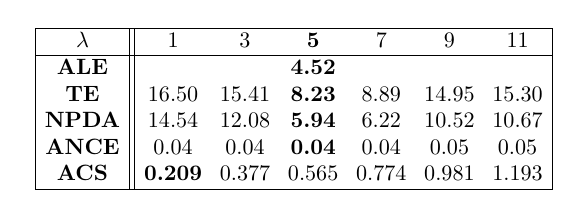
\begin{tikzpicture}[inner sep=0pt,outer sep=0pt,scale=1, every node/.style={scale=0.8}]
    % 
	\node[anchor=north west] (sim_tune) at (0, 0pt)
    {
    \setlength{\tabcolsep}{4pt}
    \begin{tabular}{|c||cccccc|}
    \hline 
    \textbf{$\lambda$} & 1 & 3 & \textbf{5} & 7 & 9 & 11 \\ 
    \hline 
    \textbf{ALE}  &  &  & \textbf{4.52} &  &  &  \\ 
    \textbf{TE}   & 16.50 & 15.41 & \textbf{8.23} & 8.89 & 14.95 & 15.30  \\ 
    \textbf{NPDA} & 14.54 & 12.08 & \textbf{5.94} & 6.22 & 10.52 & 10.67  \\ 
    \textbf{ANCE} & 0.04 & 0.04 & \textbf{0.04} & 0.04 & 0.05 & 0.05  \\ 
    \textbf{ACS}  & \textbf{0.209} & 0.377 & 0.565 & 0.774 & 0.981 & 1.193  \\ 
    \hline 
    \end{tabular}
    };       

\end{tikzpicture}
\end{minipage}
\vspace*{-0.5em}
\end{figure*}
    
\end{document}